\pagestyle{aaron}
\section{Einführung und Versuchsaufbau} \label{sec:Einfuehrung}

Inhalt dieser Belegarbeit ist die Modellierung eines inversen Pendels, welches über ein Schwungrad regelungstechnisch in der aufrechten Position stabil gehalten werden soll. \\

Diese Arbeit geht dabei im ersten Abschnitt auf den \textbf{Versuchsaufbau} und die \textbf{Modellierung} des Pendels ein. Es schließt sich eine \textbf{Sensitivitäts- und Parameteranalyse} an, über welche der Einfluss bestimmter Modellgrößen auf das Verhalten des Systems untersucht wird. \\
Nachdem das Modell aufgestellt und auf seine Eigenschaften analysiert wurde, folgt die Implementierung als Simulation in Matlab/Simulink. Dafür soll zunächst das \textbf{Aufschwingen des Pendels}. umgesetzt werden. Kann das Pendel bis in einen bestimmten Bereich um die obere Ruhelage bewegt werden, übernimmt ein \textbf{einfacher Zustandsregler}, welcher ebenfalls in dieser Arbeit entworfen wird. \\
Abschließend wird ein \textbf{Beobachter} umgesetzt, über welchen die nicht messbaren Zustände des Systems rekonstruiert werden können, um den Regler am realen Versuch in Betrieb zu nehmen.

Nachfolgend findet sich die Darstellung der Modellparameter/Konstanten zur Modellierung des Schwungrad-Pendels (siehe \autoref{tab:Tabelle1.1}).

\begin{table}[H]
    \centering
    \begin{tabular}{|lll|}
        \hline
        \rowcolor{grey}
        \textbf{Symbol}     & \textbf{Parameter}                                & \textbf{Wert/Einheit}                         \\ \hline
        $\theta$            & Winkel des Pendels                                & $\SI{}{rad}$                                  \\
        $\varphi$           & Winkel des Schwungrades                           & $\SI{}{rad}$                                  \\
        $J_{\mathrm{1}}$    & Trägheitsmoment des Pendels (+ Motorstator)       & $\SI{0.01186}{kg \cdot m^2}$                  \\
        $J_{\mathrm{2}}$    & Trägheitsmoment des Rads (+ Motorrotor)           & $\SI{0.0005711}{kg \cdot m^2}$                \\
        $c_{\mathrm{1}}$    & Reibungsfaktor des Pendels                        & $\SI{0.04}{\frac{N \cdot m \cdot s}{rad}}$    \\
        $c_{\mathrm{2}}$    & Reibungsfaktor des Rads                           & $\SI{0.0001}{\frac{N \cdot m \cdot s}{rad}}$  \\
        $m_{\mathrm{1}}$    & Masse des Pendels und Stators                     & $\SI{0.826}{kg}$                              \\
        $m_{\mathrm{2}}$    & Masse des Rads und Rotors                         & $\SI{0.583}{kg}$                              \\
        $l_{\mathrm{1}}$    & Länge vom Ursprung bis Schwerpunkt des Pendels    & $\SI{0.1053}{m}$                              \\
        $l_{\mathrm{2}}$    & Länge vom Ursprung bis Schwerpunkt des Rads       & $\SI{0.14}{m}$                                \\
        $K_{\mathrm{b}}$    & Back-End-Konstante                                & $\SI{0.0987}{\frac{V}{\frac{rad}{s}}}$        \\
        $K_{\mathrm{t}}$    & Motor-Drehmoment-Konstante                        & $\SI{0.0987}{\frac{N \cdot m}{A}}$            \\
        $R_{\mathrm{a}}$    & Widerstand der Ankerwicklung                      & $\SI{1.5562}{\Omega}$                         \\ \hline
    \end{tabular}
    \caption{Modellparameter des Schwungrad-Pendels}
    \label{tab:Tabelle1.1}
\end{table}

Ziel der Arbeit soll es sein, anhand von Beispielparametern eine effektive Regelung umzusetzen, welche später bei der Übernahme auf einen realen Versuchsaufbau einfach adaptiert werden kann. Dazu ist es wichtig ein gutes Modell umzusetzen und den Einfluss der verschiedenen Modell- und Regelparameter auf das Verhalten des Systems zu kennen. \\

\autoref{fig:Bild1.1} zeigt den modellhaften Versuchsaufbau. Das System besteht aus einem Pendel und einem Schwungrad. Das Pendel kann frei rotieren um die 0z-Achse, die senkrecht zur 0xy-Ebene steht. Das Schwungrad wird durch einen Gleichstrommotor angetrieben und dreht sich um eine Achse parallel zur 0z-Achse. Das Pendel kann durch die Reaktionskraft ausbalanciert werden, die durch das Schwungrad erzeugt wird.

\begin{figure}[H]
   \centering
   \fbox{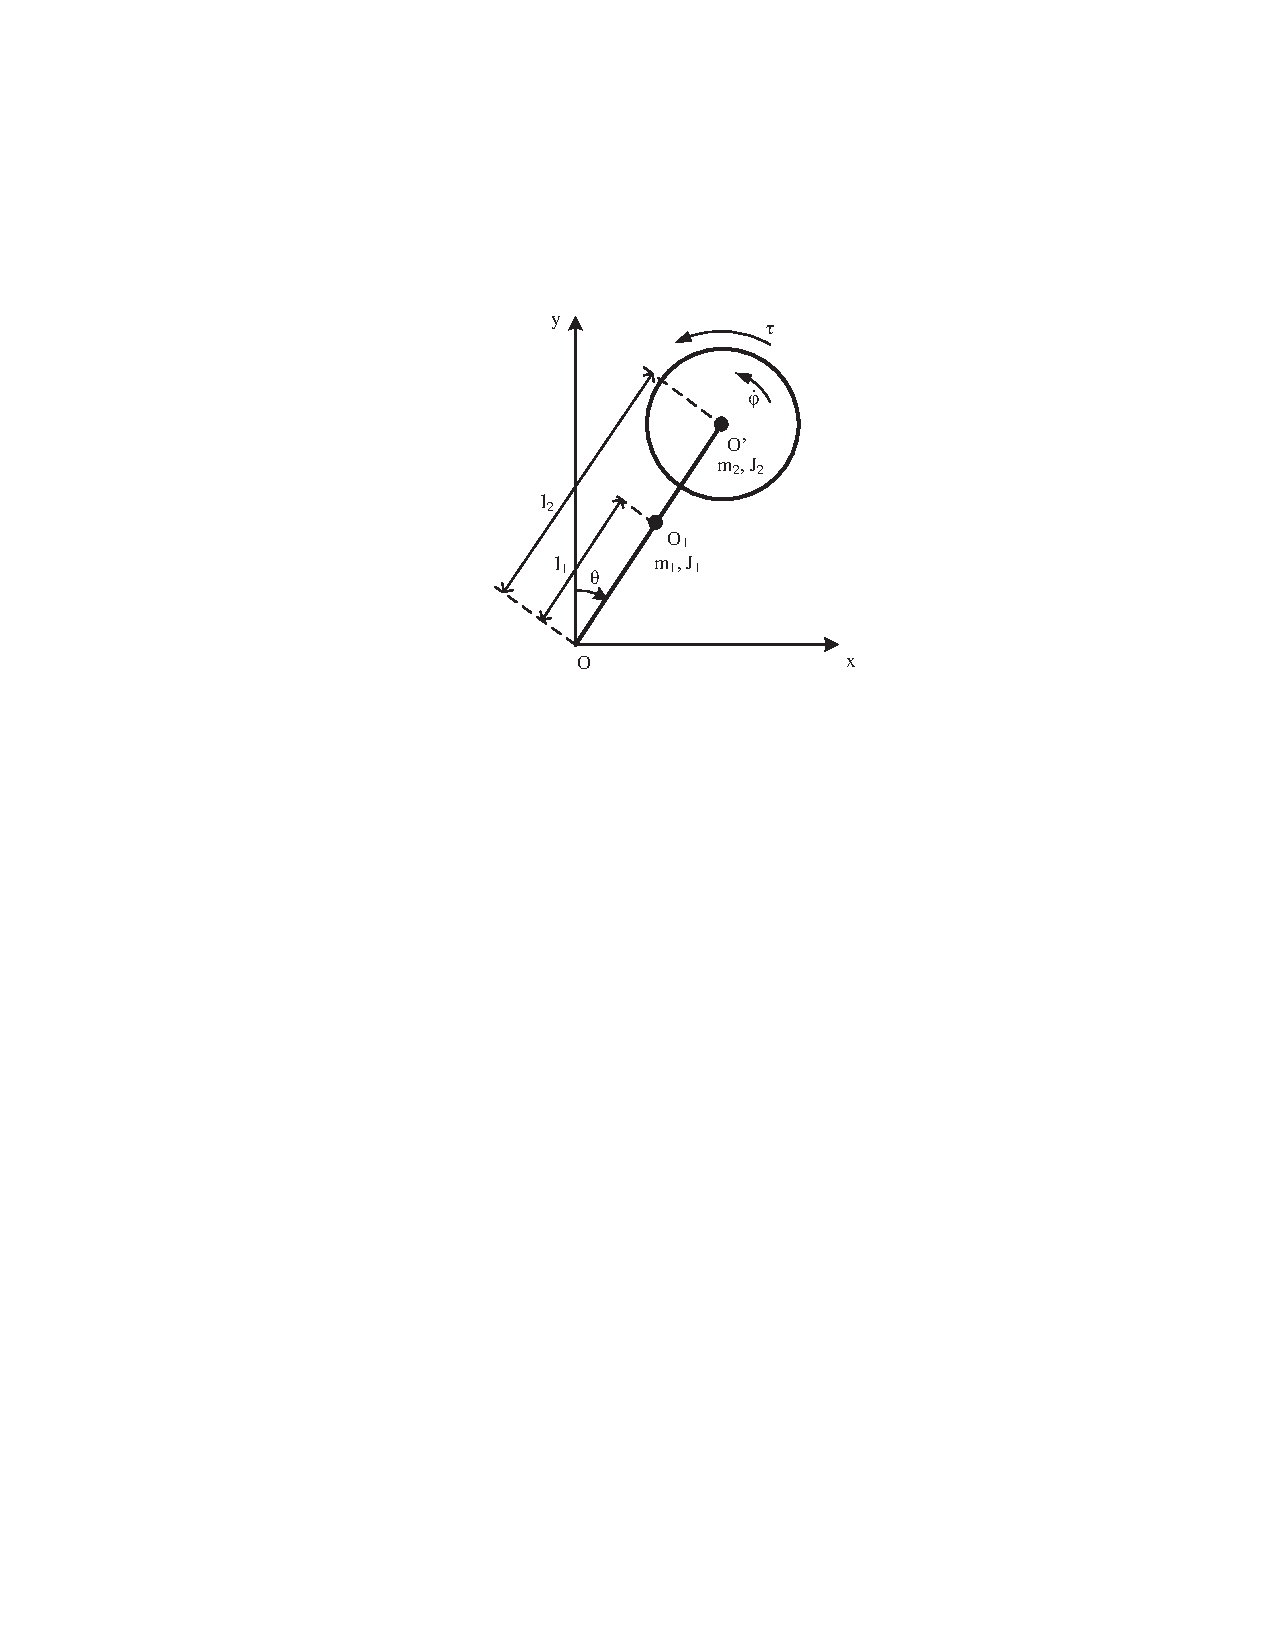
\includegraphics[width=0.4\textwidth]{Bilder/1_einfuehrung/Versuchsaufbau.pdf}}
   \caption[Modellskizze des Versuchs]{Modellskizze des Schwungrad-Pendel-Versuchs inklusive relevanter Modellparameter}
   \label{fig:Bild1.1}
\end{figure}

Weiterhin gelten folgende Voraussetzungen für das System:

\begin{itemize}
    \item Das Pendel ist frei gelagert.
    \item Der Motor (Gleichstrommaschine) ist spannungsgeregelt (bei $V_{\mathrm{m,Max}} = \SI{20}{V}$).
    \item Der Winkel ($\theta$) des Pendels und der Winkel ($\varphi$) des Schwungrades werden gemessen.
\end{itemize}

Es sind folgende Einschränkungen ermittelt/festgelegt worden:

\begin{itemize}
    \item Das Aufschwingen soll über eine schnelle Steuerung umgesetzt werden.
    \item Es soll ein Zustandsregler mit vier Zuständen ($x_{\mathrm{1}}$ bis $x_{\mathrm{4}}$) verwendet werden für die Regelung um die Ruhelage.
    \item Für die Ermittlung der Winkelgeschwindigkeiten ($\dot\theta$ und $\dot\varphi$) ist die Rekonstruktion über einen Beobachter notwendig.
\end{itemize}